O sol continua a sua ascensão no céu e a temperatura do ar está muito agradável.
Na tela azul celestial não estão desenhadas nuvens.

Mas, quando elas quando aparecem, são sempre um deleite e uma companhia para quem está na terra.

As pedras, as flores, as árvores, os animais, os insetos e até alguns humanos gostam de observá-las.

O vento sopra exalando-lhes vida e elas criam pinturas mutantes.

Os pássaros são uns privilegiados, porque podem se misturar com as nuvens.

Há sempre bandos de pássaros a voar no céu.
\bigbreak
A porta da casinha no meio do jardim abre-se.

Uma menina, de sardas no rosto, tranças no cabelo, com um vestido florido e os pés descalços, sai a correr pelo relvado.

Vem tão sorridente e cheia de alegria que o jardim, instantaneamente em comunhão, lhe sorri também.

Corre de braços abertos, como se fossem asas de gaivota, e de olhos fechados na direção do sol. E o sol inunda-a de energia.

Mas nem todos a sentem assim.

\begin{figure}[h]
    \centering
    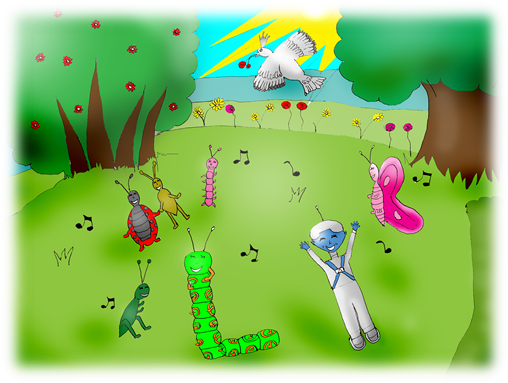
\includegraphics[width=0.85\textwidth]{ave}
\end{figure}

\bigbreak
— Fujam! – grita uma formiga – Fujam que vem lá a barafunda!
\bigbreak

E os insetos desatam a correr. Metem-se nas tocas, misturam-se nas flores e escondem-se nas árvores.

Num piscar de olhos a reunião debaixo do canteiro dos lírios fica sem nenhum bicho.

Apenas o \textbf{Eu sou Eu} permanece onde está divertindo-se com o enorme alvoroço presente.

E ri, ri muito.

A menina brinca sentada na relva, batendo as palmas e depois batendo numas mãos imaginárias à sua frente. É desta maneira que ela se entretém no jardim. Nunca está sozinha, mesmo que pareça estar. Canta e conversa com o vento, com os reflexos do sol que surgem por todos os lados e talvez com pequenos duendes invisíveis que só as crianças conseguem ver.
\bigbreak
Então \textbf{Eu sou Eu} diz:
\bigbreak
— Não vejo nenhuma barafunda. Vocês fogem do nada.

Perante esta afirmação, os insetos começam a espreitar dos seus esconderijos.

Novamente, e com muita ordem, os lugares da reunião debaixo do canteiro dos lírios vão sendo preenchidos.

O \textbf{Eu sou Eu} dá algum tempo para os mais assustados se recomporem.

A porta-voz formiguinha explica o porquê da fuga.
\bigbreak
— Sabes, nós vivemos neste jardim há muito tempo, mas, por vezes, quando estamos em grupo e somos muitos, os humanos fumigam-nos e atiram terra ou água sobre o local onde nos encontramos. Às vezes conseguimos escapar, outras vezes não. Eles acham que somos prejudiciais e dizem que somos pragas! Mal sabem eles que cuidamos e revolvemos a terra dos seus jardins.
\bigbreak
O \textbf{Eu sou Eu} levanta-se da pedra onde está sentado, abre os braços imitando asas de gaivota e corre, tal como a menina, pelo jardim. E só para junto aos insetos. E com muita doçura diz-lhes:

— Isso não devia acontecer! Mas lembrem-se de que grande parte dos humanos neste mundo são um pouco adormecidos. Muitos não vivem a Unidade, como eu no meu planeta e vocês nas vossas colónias.

Eles, desde muito pequenos e conforme vão crescendo e tornando-se adultos, ganham certos hábitos e acreditam que podem mandar em tudo e controlar tudo e todos à sua volta. Puro engano. Mas nem todos são assim. As crianças, por exemplo, são puras, sem crenças. Vivem no momento presente, o que lhes permite estar em harmonia. Mas elas nem sonham que é assim, porque o fazem NATURALMENTE. Brincam descontraídas e não têm maldade. Garanto que a menina não vai fumigar ou afogar nenhum de vocês. A vida para ela é uma Simples Brincadeira.
\bigbreak
\textbf{Eu sou Eu} tem razão.

As crianças são simples, não têm medo. Mesmo que se sujem por fora, permanecem limpas por dentro.

O seu coração é grande e é com ele que observam o mundo. Os seus olhos verdadeiros estão dentro do peito e não na cabeça!

Interagem com o que as rodeia de uma forma inocente e fluida. Pode ser feio, bonito, grande ou pequeno, preto, branco ou outra cor, sujo ou asseado, novo ou quebrado. Elas arranjam continuamente maneira de encontrar Beleza e Alegria em tudo.

São sempre Espontâneas, Diretas e Transparentes no que falam e fazem, o que por vezes, ou melhor, muitas vezes, os humanos adultos ficam sem saber o que lhes responder.

A linguagem das crianças é a do coração, livre, leve.

Mas com o tempo, com a educação que lhes é oferecida, com as regras e crenças da sociedade em que vivem, vão crescendo e sendo formatadas, vão-se adulterando e ficando aprisionadas nas coisas complicadas.

Pois tudo o que está fora do Coração é complexo.

Ao contrário das crianças, os adultos geralmente não fluem com a Vida e são muito enferrujados mentalmente. E complicam o que não é complicado.

— Joana! Joaninha, onde estás? – uma voz altifalante sai da casa e chega aos ouvidos de todo o jardim. A mãe da menina está a chamá-la.
\bigbreak
A Joana, que curiosamente tem nome de inseto, não se apercebe e continua a brincar com o seu amigo invisível. Rebola, dá cambalhotas, e faz com que os seus pezinhos nus deslizem na relva, apreciando a frescura, ou talvez, apenas sentindo as cócegas.

Ela ri sem parar, como se uma Onda de Vida subisse pelos seus pés.

— Joana!! És surda?! – grita novamente a mãe.
\bigbreak
Não, a menina não é, nem está surda e só neste instante fica atenta ao chamamento.

\begin{figure}[h]
    \centering
    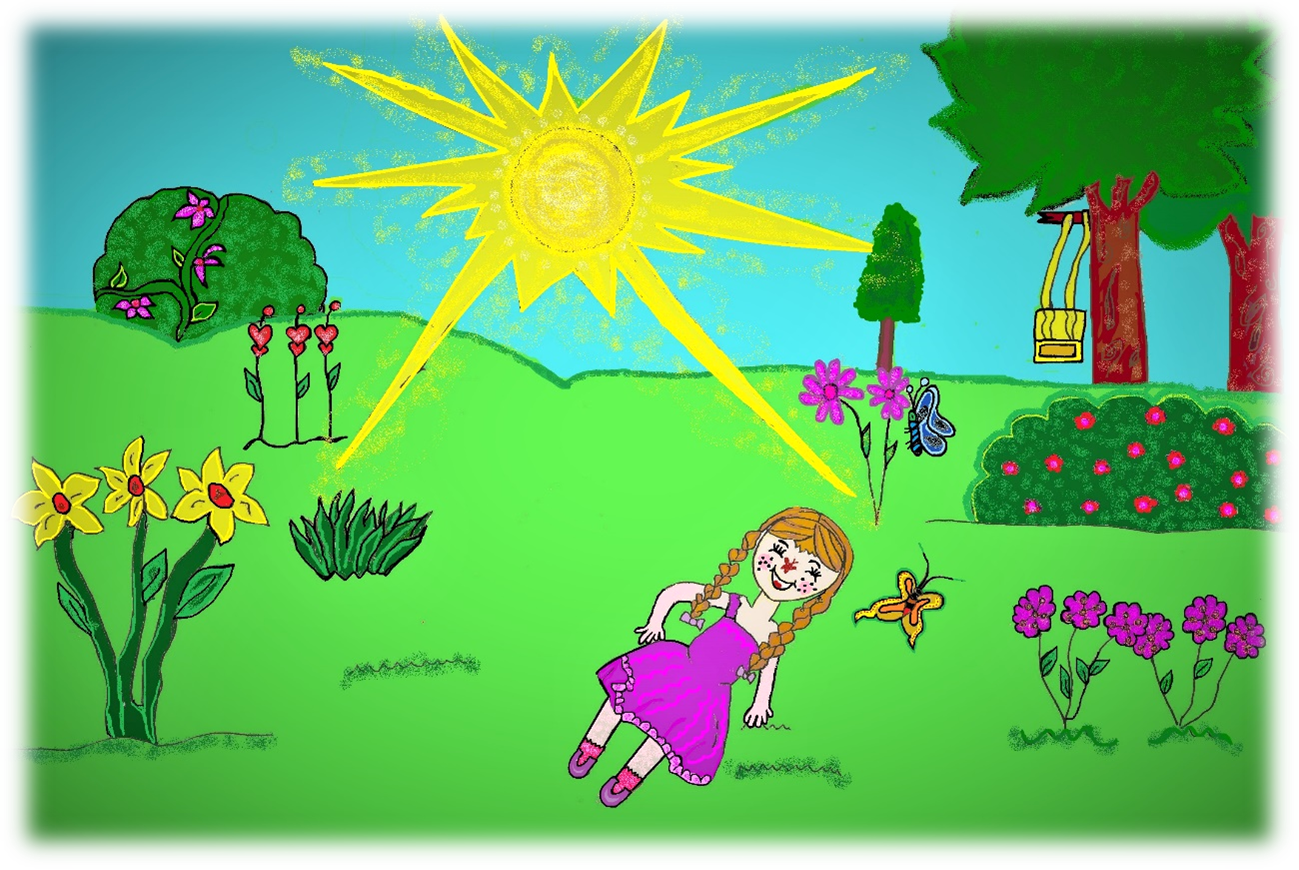
\includegraphics[width=0.85\textwidth]{menina}
\end{figure}

Levanta-se da cambalhota que acaba de dar e corre para dentro de casa. A porta fecha-se.
\bigbreak
O jardim está outra vez silencioso.

Mas é um silêncio que integra na sua plenitude:

O sussurrar do vento – Fiuuuuuuu!

O sibilar dos insetos – Ssssssssssss!

E o Ploc! Ploc! Ploc! de algumas bolas de sabão que só agora tocam o chão.

O sol continua o seu caminho entre o nascente e o poente.

É hora de almoço.
